\chapter{Descrizione del modello}

\section{Framework adottato}

\todo{reference} Mesa è un framework in Python usato per la modellazione basata su agenti (ABM). Permette di creare il modello con componenti \textit{built-in} come griglie spaziali e scheduler di agenti, e di visualizzare i componenti del modello con un'interfaccia browser. Sfruttando Mesa è possibile definire sia l'ambiente che gli agenti estendendo le relative classi messe a disposizione dal framework. Mesa infine comprende strumenti per l'analisi del modello creato.

Nel nostro modello di supermercato, il modello vero e proprio di Mesa è la classe \textbf{Supermarket} e gli agenti sono i clienti, classe \textbf{Customer}, e le casse, classe \textbf{CashDesk}. 

\section{Sistema}
Supermercato non predicibile, presente una componente stocastica.

Il sistema è eterogeneo, due tipi di agenti. Sistema multiagente.

Come comunicano

Come avviene l'interazione

Descrizione dell'ambiente

\section{Agente di tipo Cliente}
I clienti sono gli agenti principali che compongono il modello e interagiscono con l'ambiente per raggiungere l'obiettivo di fare la spesa; per portare a termine questo compito l'agente esegue alcuni macro-step in cui è necessaria anche una fase di pianificazione e valutazione della bontà (\textit{utility function}) della scelta adottata in alcune di queste.

\subsection{Workflow}
I macro-step che l'agente deve seguire per il raggiungimento del goal, che coincidono con gli stati associati all'agente durante la simulazione, sono:

\begin{enumerate}
	\item \textbf{Attesa all'entrata del supermercato}: in questo stato il cliente si mette in attesa finchè non è possibile entrare nel supermercato. \todo{Esperimenti sul covid}
	\item \textbf{Fase di shopping}: il cliente è entrato e può iniziare a "fare la spesa", con questo si intende raggiungere il numero di prodotti desiderato, infatti nella simulazione viene considerato il \textit{basket size}, un'astrazione del carrello modellato attraverso un numero interno. Il basket size è il target da raggiungere nella fase di shopping, a ogni step il numero di prodotti aumenta di una certa quantità (la velocità di shopping è un parametro del modello descritto nella sezione \ref{model:parameters}). 
	
	La basket size viene generata stocasticamente secondo una distribuzione esponenziale governata dal parametro $\lambda = 0.07361$. La scelta di questo parametro viene giustificata nella sezione \ref{model:parameters}. 
	
	\item \textbf{Scelta della coda}: in questo stato il cliente ha finito di fare la spesa e vuole mettersi in coda ad una cassa. Dal momento che sono disponibili più code e ognuna di queste avrà molto probabilmente altri clienti già in coda, il cliente deve scegliere in quale coda andare in base alla coda che lui considera migliore.
	
	Formalmente viene definita una strategia di scelta della coda in base a una funzione: la \textit{utility function}. Il cliente sceglie quindi la coda che minimizza questa funzione:

	\begin{equation}
		q^* = \operatorname*{argmin}_{q \in Q} f(q) \label{eq:strategy}
	\end{equation}
	dove $Q$ è l'insieme delle code dedicate e $f$ varia a seconda del tipo di strategia che il cliente può utilizzare, ognuna delle quali modella una diversa strategia per la scelta della coda.

	\item \textbf{Attesa in coda e jockeying}: una volta che il cliente ha scelto la coda deve aspettare il proprio turno per essere servito. Nel lavoro di Tomasz Antczak e altri \cite{article1} viene suggerito come sviluppo futuro lo studio del fenomeno di \textit{jockeying}: con questa espressione si intende cambiare la coda che è stata scelta inizialmente in quanto un'altra risulta essere più conveniente, ad esempio perchè più scorrevole.
	
	Ad ogni timestamp l'agente considera le due code adiacenti (parametro spiegato nella sezione \ref{model:parameters} e scelto a priori per il modello) alla propria e per ognuna di queste ricalcola la coda migliore secondo la \ref{eq:strategy}. A questo punto l'agente valuta se per lui è conveniente cambiare la coda o rimanere in quella dove è già presente. Si noti come per effettuare questo confronto è necessario utilizzare l'approccio della \ref{eq:strategy} sulla coda in cui l'agente è in quel momento, andando ad escludere i clienti che si sono inseriti in coda dopo di lui. Una volta fatta questa valutazione, nel caso in cui sia per lui conveniente cambiare coda, il cliente la cambia in modo stocastico secondo una certa distribuzione di probabilità spiegata nella sezione \ref{implementation:intro}, che è maggiore più il cambio di coda risulta conveniente.
	
	La scelta modellistica di effettuare jockeying stocasticamente e in funzione dell'effettivo guadagno di tempo è stata fatta per cercare di avere una rappresentazione il più fedele possibile al mondo reale. Infatti nella realtà un cliente al supermercato potrebbe scegliere di non cambiare la coda nel momento in cui ha un guadagno minimo in quanto questo richiede uno sforzo fisico che non tutti vogliono spendere nella realtà. Inoltre questa operazione richiede che gli agenti controllino continuamente le casse vicine, anche questo non è necessariamente vero in quanto dispendioso di energia. Infatti nel lavoro di Tomasz Antczak e altri \cite{article1} viene fatto notare come questo comportamento non sia molto frequente, tuttavia seppur essendo poco frequente noi lo consideriamo un fattore importante da modellare, adottando le dovute precauzioni e sfruttando la stocasticità dell'azione.
	
	\item \textbf{Attesa alla cassa}: in questa fase il cliente è arrivato alla cassa, essendo arrivato con lo stato precedente in prima posizione della coda. Da questo punto in poi verrà servito dall'agente di tipo cassa che avrà la responsabilità di processare il basket size del cliente. Dal momento che ci sono diversi tipi di casse, questa fase dipende dall'agente di tipo cassa e non dal cliente. Il cliente deve attendere la fine dell'elaborazione della spesa e quindi uscire dal negozio.
\end{enumerate}

Il workflow dell'agente di tipo cliente viene astratto e riassunto da questa immagine:


\begin{figure}[htp!]
	\centering
	\hspace*{3cm}
	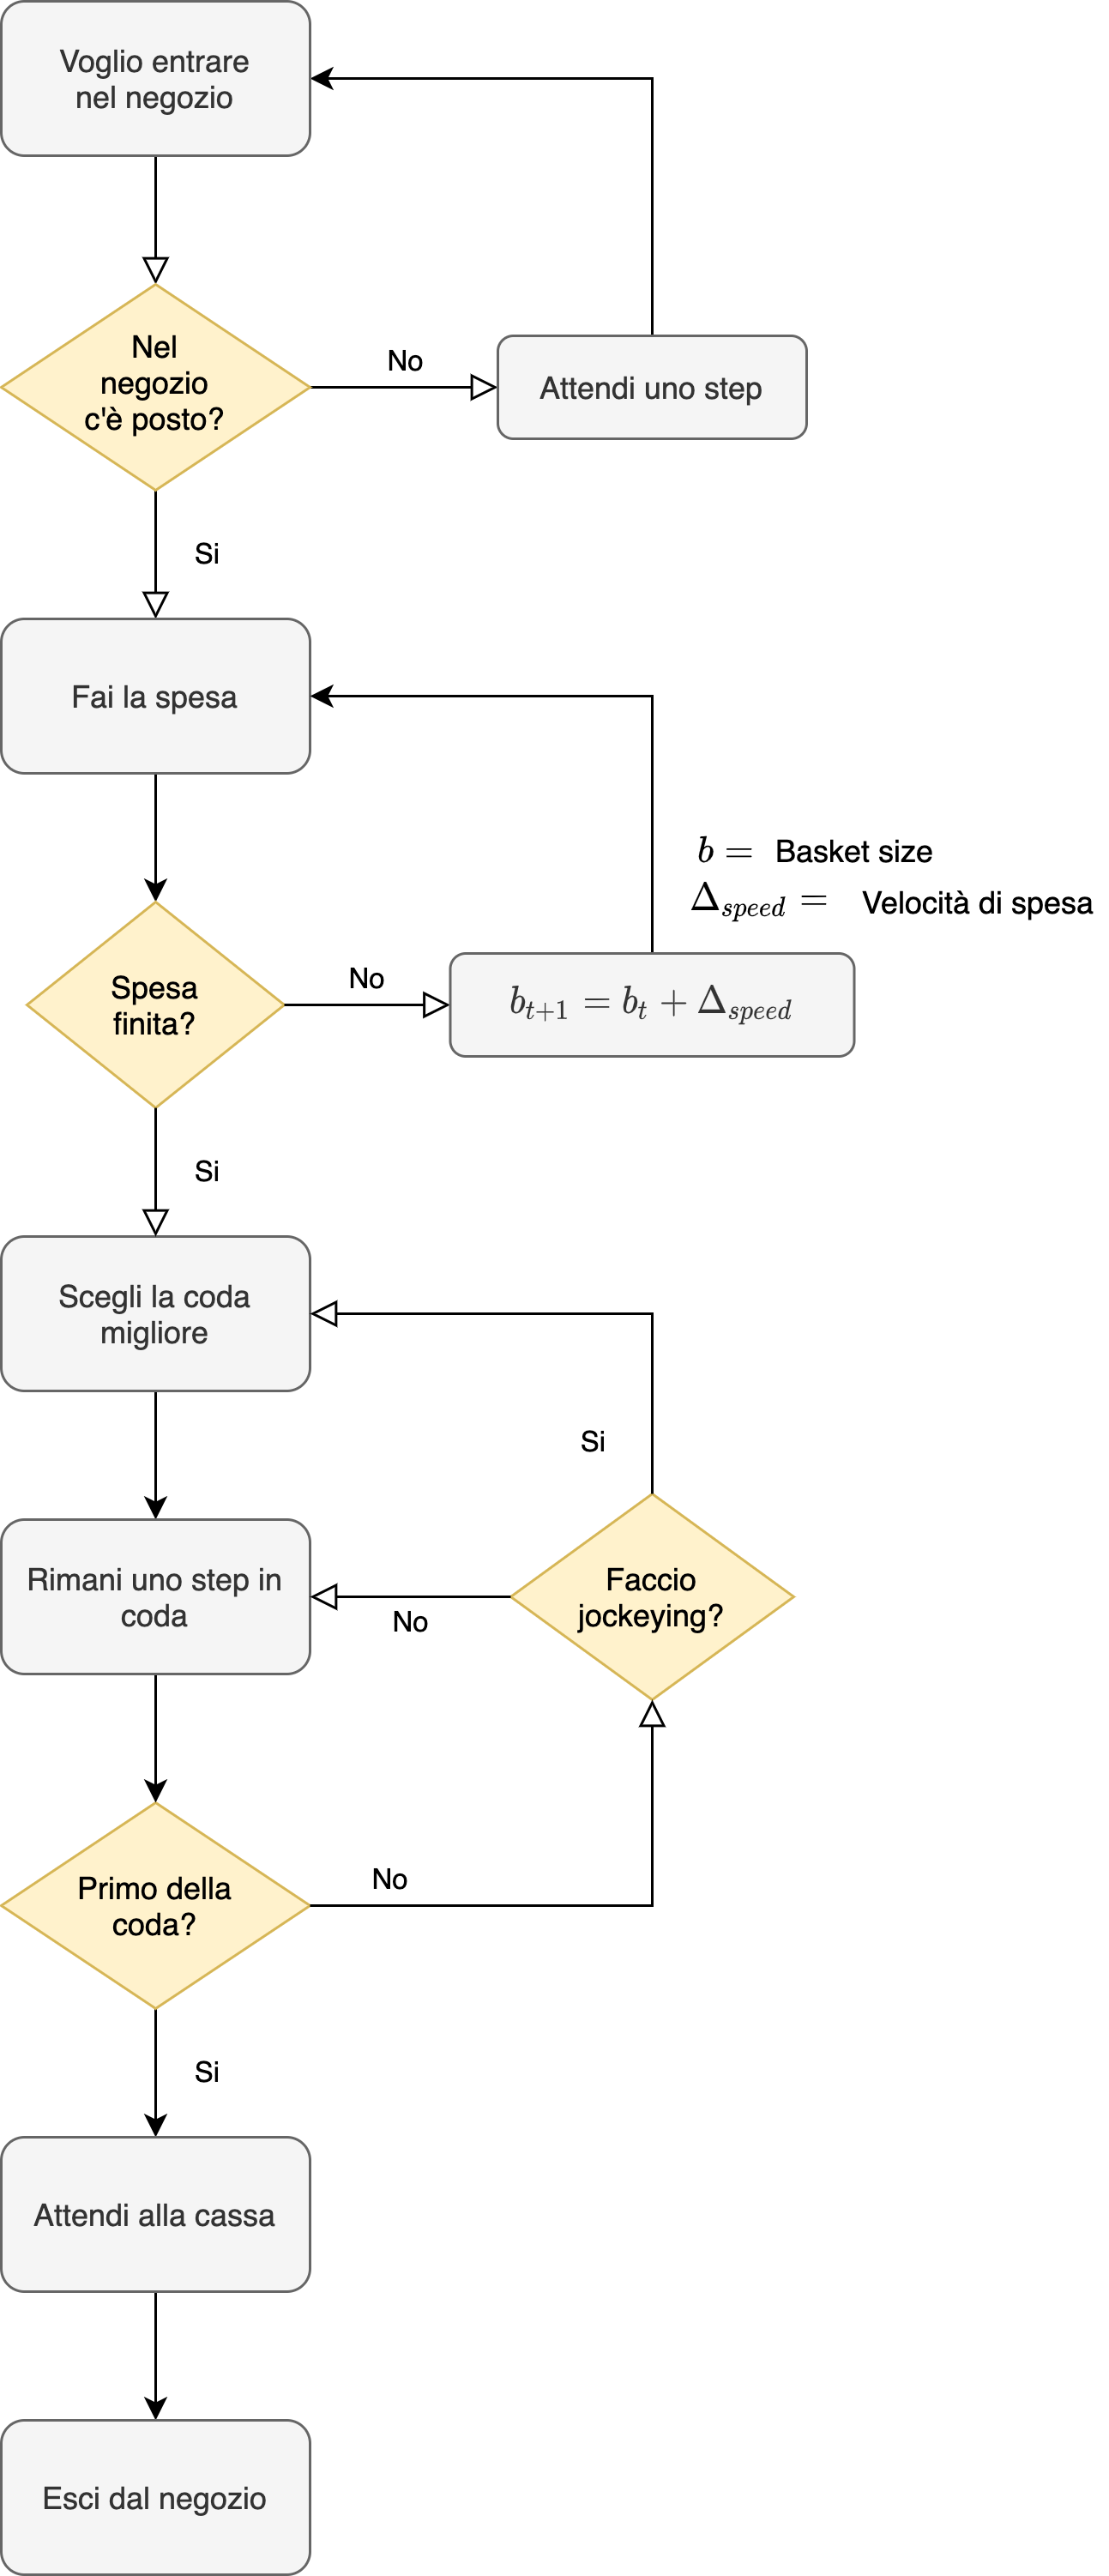
\includegraphics[width=8cm]{"images/workflow_customer.png"}
	\caption{Workflow dell'agente di tipo customer.}
	\label{fig:workflow_customer}
\end{figure}


\subsection{Architettura}

\section{Agente di tipo Cassa}
\label{model:cashdesks}


Gli agenti di tipo cassa hanno l'unica funzione di servire i clienti che si mettono in coda per pagare la spesa; sono di 4 tipi e differiscono per modalità di elaborazione della spesa del cliente e per velocità.

\begin{enumerate}
\item \textbf{Cassa standard}: questa cassa rappresenta la normale cassa che si trova solitamente in tutti i supermercati, all'interno della quale lavora un cassiere che si occupa di passare i prodotti del carrello del cliente sul nastro.
 
Il tempo di servizio di un cliente per questo tipo di cassa è formato da due tempi diversi: il \textbf{transaction-time}, che è il tempo vero e proprio durante il quale avviene la transazione, e il \textbf{break-time}, che è il tempo che passa tra il servizio di un cliente e di un altro ed include anche la fase in cui il cliente insacchetta i prodotti acquistati. Il transaction-time è stato stimato con una regressione di potenza e il break-time con una distribuzione Gamma. In particolare, per un cliente $c_i \in q$, i due tempi sono calcolati in questo modo:

\begin{equation}\label{eq:transaction-time-standard}
\text{transaction-time}_i = e^{a log(\text{basket-size}(c_i)) + b}
\end{equation}
\begin{equation}\label{eq:break-time-standard}
\text{break-time}_i = \frac{\beta^{\alpha} \text{basket-size}(c_i)^{\alpha - 1} e^{- \beta \text{estimate-basket-size}(c_i)}}{\Gamma (\alpha)}
\end{equation}

Dove $\Gamma$ è la funzione \textbf{gamma} e corrisponde a:

\begin{equation}
\Gamma (z) = \int_{0}^{\infty} x^{z-1} e^{-x} dx \;\; \forall z \in \mathbb{C}
\end{equation}

Queste stime sono state prese dall'articolo \cite{article1} e in particolare i parametri $a,b,\alpha ,\beta \in \mathbb{R}$ sono:

\begin{equation}
a = 0.6984, \;\; b = 2.1219, \;\; \alpha = 3.074209, \;\; \beta = \frac{1}{4.830613}
\end{equation}

\item \textbf{Cassa self-service}: alla cassa self-service il cliente provvede da solo al passaggio dei prodotti del carrello allo scanner, per cui non è presente un cassiere. Si suppone che il cliente non sia veloce quanto un cassiere esperto a passare i prodotti sullo scanner, per questo la velocità di processing per questa cassa è stata divisa per un fattore $1.5$, uno dei parametri descritti nella sezione \ref{model:parameters}. 

Anche in questo caso il tempo di servizio è diviso in transaction-time e break-time, solo che, a differenza della cassa normale, il break-time risulta più lungo in quanto il cliente inizia ad insacchettare solamente dopo aver passato i prodotti allo scanner, invece nella cassa standard può iniziare già mentre il cassiere passa i prodotti. In questo caso, dunque, il transaction-time e il break-time sono stati stimati entrambi con una regressione di potenza:

\begin{equation}\label{eq:transaction-time-self-service}
\text{transaction-time}_i = e^{a log(\text{basket-size}(c_i)) + b}
\end{equation}
\begin{equation}\label{eq:break-time-self-service}
\text{break-time}_i = e^{c log(\text{basket-size}(c_i)) + d}
\end{equation}

I parametri in questo caso sono:

\begin{equation}
a = 0.6725, \;\; b = 3.1223, \;\; c = 0.2251, \;\; d = 3.5167
\end{equation}

\item \textbf{Cassa self-scan}: la cassa self-scan si differenzia totalmente dalle prime due descritte, il cliente che voglia utilizzarla infatti, deve deciderlo già al momento dell'entrata nel supermercato, in quanto deve scannerizzare i prodotti man mano che fa la spesa; una volta arrivato alla cassa self-scan, egli deve semplicemente effettuare il pagamento, saltando quindi le fasi di scanner e insacchettamento che caratterizzano le casse standard e self-service. La velocità di elaborazione della spesa in questo caso è praticamente nulla, in particolare un cliente che inizia il pagamento a una cassa self-scanner, lo termina allo step successivo; il tempo di pausa per questa cassa è ugualmente nullo, dato che un cliente paga ed entra immediatamente nella fase di uscita dal negozio.

Chiaramente per evitare che vengano rubati prodotti, i supermercati decidono di effettuare dei controlli random sui clienti che scelgono di usare le casse self-scan. A questo scopo è stata implementata la cassa di tipo riservato.
\item \textbf{Cassa riservata}: questa cassa è identica nel funzionamento a una cassa standard, ciò che cambia è che è riservata alla rilettura della spesa dei clienti self-scan, che avviene in maniera random. Nel momento in cui un cliente si approccia ad una cassa self-scan, viene estratto un numero che determina la \textbf{rilettura parziale} o la \textbf{rilettura totale} della sua spesa;
la rilettura parziale consiste nell'estrazione di 10 prodotti dal carrello e nella verifica che essi appartengano alla lista contenuta nello scanner del cliente, invece la rilettura totale consiste appunto nella rilettura completa della spesa di esso. Le probabilità di rilettura sono parametri del modello ed attualmente corrispondono allo $0.75 \%$ per la rilettura parziale e allo $0.25 \%$ per la rilettura totale.

Il funzionamento e i tempi di servizio sono esattamente gli stessi della cassa standard, considerando un basket-size completo per la rilettura totale e un basket-size di soli 10 elementi per la rilettura parziale.
\end{enumerate}

Tutti i tipi di cassa attraversano 3 fasi: fase di attesa di un nuovo cliente, fase di elaborazione della spesa del cliente, fase di completamento della transazione.

\subsection{Workflow}

\paragraph{Cassa standard}

Il workflow della cassa standard viene riassunto nell'immagine:

\begin{figure}[htp!]
	\centering
	\hspace*{3cm}
	
\includegraphics[width=8cm]{"images/doggo.jpg"}
	\caption{Workflow dell'agente di tipo cassa standard.}
	\label{fig:workflow_customer}
\end{figure}

\paragraph{Cassa self-service}

Il workflow della cassa self-service viene riassunto nell'immagine:

\begin{figure}[htp!]
	\centering
	\hspace*{3cm}
	
\includegraphics[width=8cm]{"images/doggo.jpg"}
	\caption{Workflow dell'agente di tipo self-service.}
	\label{fig:workflow_customer}
\end{figure}

\paragraph{Cassa self-scan}

Il workflow della cassa self-scan viene riassunto nell'immagine:

\begin{figure}[htp!]
	\centering
	\hspace*{3cm}
	
\includegraphics[width=8cm]{"images/doggo.jpg"}
	\caption{Workflow dell'agente di tipo cassa self-scan.}
	\label{fig:workflow_customer}
\end{figure}

\paragraph{Cassa riservata}

Il workflow della cassa riservata viene riassunto nell'immagine:

\begin{figure}[htp!]
	\centering
	\hspace*{3cm}
	
\includegraphics[width=8cm]{"images/doggo.jpg"}
	\caption{Workflow dell'agente di tipo cassa riservata.}
	\label{fig:workflow_customer}
\end{figure}

\subsection{Architettura}

\section{Ambiente}
La classe \textbf{Supermarket} si occupa di inizializzare la griglia che verrà poi mostrata in fase di simulazione sull'interfaccia, inizializzare le casse, l'ambiente e i clienti.

Per inizializzare la griglia, l'ambiente viene diviso in zone: zona d'entrata, zona di shopping, zona casse normali, zona casse self-service, zona casse self-scan. Questa divisione permette una gestione più semplice dello spazio e dei movimenti degli agenti. Ogni zona ha come parametri la dimensione o il numero di casse che deve contenere, questi parametri vengono inizializzati nella classe \textbf{main}, come si vedrà nella prossima sezione.

Ogni zona è responsabile della propria costruzione, ovvero del proprio collocamento nella griglia dell'interfaccia in base alle proprie dimensioni ed eventualmente del posizionamento delle casse che contiene. Inoltre ogni zona è responsabile dei movimenti dei clienti: se un cliente vuole muoversi da una zona all'altra oppure mettersi in coda nelle casse di una zona, è la zona di destinazione che fornisce il metodo per posizionarsi correttamente in essa.

\todo{Parlare di quanto dura uno step e quanto dura una simulazione} Ad ogni step della simulazione, il modello crea dei clienti secondo la distribuzione data (si veda la sezione \ref{model:parameters}) e li posiziona nella \textbf{Entering Zone} del supermercato in coordinate random, dunque si occupa della attivazione e disattivazione delle casse standard in base al numero di clienti presenti nel negozio in quello step, secondo dei parametri che si vedranno nella prossima sezione. Quindi il modello chiama gli scheduler degli agenti, clienti e casse, e fa eseguire i loro step.

\subsection{Caratteristiche dell'ambiente}
- Accessibile vs. Inaccessibile
- Deterministico vs. Non-deterministico
- Episodicità vs. Non-episodicità
- Statico vs. Dinamico
- Discreto vs. Continuo

\subsection{Interazione tra agenti}

\section{Considerazioni sul modello}

Il modello é stato sviluppato cercando di renderlo flessibile per
permettere con semplicitá future espansioni e cambiamenti. Gli aspetti
piú dinamici del modello, quindi il comportamento degli agenti e le
varie modalitá di scelta di una coda e la capacitá di un agente
Customer di effettuare Jockeying sono stati realizzati lasciando
all'utilizzatore piena possibilitá di modifica, ampliazione o di non
utilizzo. A livello di architettura del software questo si traduce
nell'implementazione dei pattern:

% TODO forse aggiungere link a pattern GOF, non so come citare correttamente
\begin{itemize}
\item \textbf{Strategy}: Usato per definire diverse modalitá di scelta
  della coda e diversi comportamenti di Jockeying. Nuovi comportamenti
  possono essere aggiunti rispettando un'interafaccia
  standard. Permette inoltre se necessario cambiamenti di
  comportamento a run time.
\item \textbf{State}: Usato per definire tramite una macchina a stati
  finiti i comportamenti degli agenti Customer e Cashdesk. Nuovi stati
  possono essere aggiunti con facilitá e collegati ad altri stati
  tramite transizioni. La divisione in stati rende semplice ragionare
  sul comportamento di un agente.
\end{itemize}

\section{Parametri del modello}
\label{model:parameters}

Casse adiacenti considerate

Inizializzazione della griglia e parametri per creare casse (numero casse, coda condivisa o no, velocità di processing e parametro per rallentare la velocità della self-service), customer, basket size (analisi dei dati di Gianluca).

\subsection{Basket size}
Citare paper con i dati.

\section{Workflow degli agenti}

\todo{non lo abbiamo mica detto sopra?}

Steps: ad ogni step entrano clienti in base alla distribuzione data come parametro; ad ogni step le casse decidono se aprire o chiudere in base al numero di clienti presenti; mettere grafici dei comportamenti e degli stati dei clienti e delle casse (quindi descrizione in dettaglio di ogni cassa e tipo di coda, di ogni stato della cassa e del cliente).